\begin{figure}
\centering
\begin{tabular}{ccc}
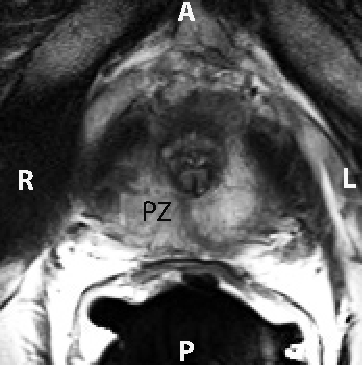
\includegraphics[width=0.29\linewidth]{figs/mr_anatomy/T2_apex} &
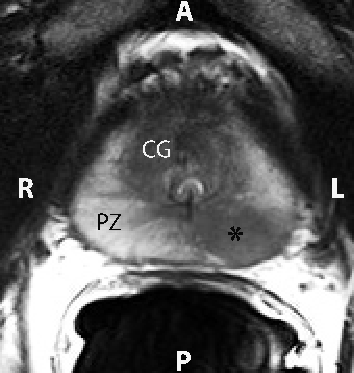
\includegraphics[width=0.275\linewidth]{figs/mr_anatomy/T2_midgland} &
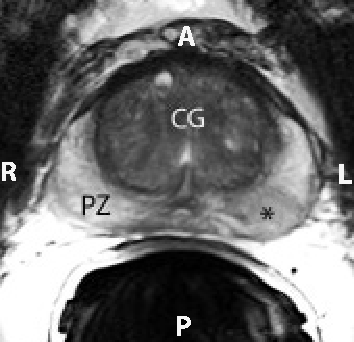
\includegraphics[width=0.3\linewidth]{figs/mr_anatomy/T2_base} \\
(a) MR T2WI Apex & (b) MR T2WI Mid-gland & (c) MR T2WI Base \\
\end{tabular}
\caption{Axial T2-weighted MR images of the prostate show the apex (a),
    mid-gland (b), and base (c).  The peripheral zone (PZ) is of higher signal
    intensity than the central gland (CG), the latter which is composed of the
    central zone and the transitional zone. The apex (a) is composed mostly of
    PZ glandular tissue and the urethra is seen at the level of the mid-gland as
    an inverted ``U'' (b). Note the area of hypointense signal in the
    peripheral zone at the mid-gland and base (asterisk, b and c), which
    represents a prostatic tumor.  The posterior (P) aspect of the prostate is
    adjacent to the endorectal coil, and the right (R)-to-left (L) extent of
    the prostate is referred to as the lateral-to-lateral axis in the subsequent
    analysis.}
\label{fig:mr_anatomy} 
\end{figure}
